\documentclass[11pt]{article}

% ----- preamble (matches the other picture books in this project) -----
\usepackage[a4paper,margin=1.8cm]{geometry}
\usepackage{amsmath,amssymb}
\usepackage{array}
\usepackage{booktabs}
\usepackage{tikz}
\usepackage{tikz-cd}
\usetikzlibrary{arrows.meta,positioning,calc,fit,backgrounds,
  shapes.geometric,chains,decorations.pathreplacing,decorations.markings}
\usepackage[most]{tcolorbox}
\usepackage{parskip}
\usepackage{xcolor}

\definecolor{ink}{RGB}{40,40,40}
\definecolor{soft}{RGB}{245,245,248}
\definecolor{kas}{RGB}{30,110,190}
\definecolor{grn}{RGB}{30,140,80}
\definecolor{red2}{RGB}{200,50,50}

% the three brick colours used across this project's picture books
\definecolor{faceL}{RGB}{30,140,80}   % linearized trace  L
\definecolor{faceF}{RGB}{200,140,0}   % Frobenius / doubling  F
\definecolor{faceC}{RGB}{130,70,170}  % cyclotomic coset bookkeeping  C
\definecolor{faceX}{RGB}{30,110,190}  % categorical loop  X

\newtcolorbox{note}[1][]{colback=soft,colframe=ink,boxrule=0.4pt,
  arc=2pt,left=6pt,right=6pt,top=4pt,bottom=4pt,#1}
\newtcolorbox{leanbox}[1][]{colback=black!4,colframe=black!55,boxrule=0.4pt,
  arc=1.5pt,left=5pt,right=5pt,top=3pt,bottom=3pt,#1}
\newtcolorbox{verdict}[1][]{colback=grn!7,colframe=grn!65,boxrule=0.7pt,
  arc=2pt,left=7pt,right=7pt,top=5pt,bottom=5pt,#1}
\newtcolorbox{caveat}[1][]{colback=red2!6,colframe=red2!55,boxrule=0.6pt,
  arc=2pt,left=7pt,right=7pt,top=5pt,bottom=5pt,#1}

\tikzset{
  vtx/.style={circle,draw=ink,fill=soft,minimum size=6.5mm,font=\small,inner sep=0pt},
  fld/.style={circle,draw=faceF,fill=faceF!12,minimum size=6.5mm,font=\small,inner sep=0pt},
  obj/.style={draw=ink,rounded corners=3pt,fill=soft,inner sep=5pt,font=\small,align=center},
  brick/.style={draw=ink,rounded corners=2pt,inner sep=6pt,font=\small,align=center,
    minimum height=13mm},
  arr/.style={-{Stealth[length=2.4mm]},thick},
  badge/.style={circle,inner sep=0pt,minimum size=3.8mm,font=\scriptsize\bfseries,text=white},
}
\newcommand{\bL}{\tikz[baseline=-0.6ex]\node[badge,fill=faceL]{L};}
\newcommand{\bF}{\tikz[baseline=-0.6ex]\node[badge,fill=faceF]{F};}
\newcommand{\bC}{\tikz[baseline=-0.6ex]\node[badge,fill=faceC]{C};}
\newcommand{\bX}{\tikz[baseline=-0.6ex]\node[badge,fill=faceX]{$\otimes$};}

\newcommand{\tr}{\operatorname{tr}}
\newcommand{\Tr}{\operatorname{Tr}}
\newcommand{\id}{\mathrm{id}}
\newcommand{\gcdd}{\operatorname{gcd}}
\newcommand{\lc}[1]{\texttt{\small #1}}
\newcommand{\ck}{\textcolor{grn}{\checkmark}}
\newcommand{\notlean}{\textcolor{red2}{$\circ$}}
\newcommand{\FF}{\mathbb F}

\title{\vspace{-1.5cm}\textbf{One Categorical Pattern, the Whole Dobbertin Paper?}\\[3pt]
\large Reading \emph{Kasami Power Functions, Permutation Polynomials and Cyclic
Difference Sets}\\ through the single evaluation/coevaluation loop \bX\\[2pt]
\normalsize \bL~linearized trace \quad \bF~Frobenius \quad \bC~cyclotomic cosets
\quad \bX~categorical trace}
\author{\small An exploration for the \texttt{Equation1} Lean\,/\,Mathlib formalisation}
\date{}

\begin{document}
\maketitle
\vspace{-1.0cm}

\begin{note}
\textbf{The question.} \emph{The categorical pattern is the abstract shape of all
three gadgets \bL\,\bF\,\bC. If the paper's results all build from the three
gadgets, do they all build from this one category-theory pattern of evaluation
and coevaluation? Could the \emph{entire} Dobbertin paper be built from this sole
pattern?}

\smallskip
\textbf{The short honest answer.} As an \emph{organising lens}: to a remarkable
degree, yes. The single move --- \emph{coevaluation opens a loop, insert a map,
evaluation closes it, keep what returns} --- is exactly the trace, and every
recurring device in the paper is that one move in a costume: \bF\ is the inserted
map, \bL\ is the closed loop, \bC\ are the surviving loops, and (the extra hinge
this note adds) the additive character $\psi(x)=(-1)^{\Tr(x)}$ that runs the
whole difference-set half of the paper is itself an evaluation pairing of $L$
with its dual. \emph{As a literal derivation}: no. The loop makes ``trace = sum
around the Frobenius orbit'' inevitable and reorganises the paper cleanly, but
several results (the Fibonacci recursion for the inverse, the Gau\ss/Jacobi-sum
2-rank computations, the difference-set proof itself) carry genuine extra
mathematics that the bare pattern does not hand you for free. Boxes marked \ck\
are backed by \lc{sorry}-free Lean declarations in \lc{Equation1/}; \notlean\
marks material outside this formalisation.
\end{note}

%======================================================================
\section{The one pattern, restated}

In a monoidal category with duals, every object $V$ carries a coevaluation
$\eta:I\to V\otimes V^{*}$ and an evaluation $\varepsilon:V^{*}\otimes V\to I$.
The \emph{trace} of $f:V\to V$ is the single composite that closes the wire into
a loop, with $f$ (or its $k$-th power) inserted:
\[
\tr(f^{k}):\; I \xrightarrow{\ \eta\ } V\otimes V^{*}
        \xrightarrow{\ f^{k}\otimes\id\ } V\otimes V^{*}
        \xrightarrow{\ \mathrm{swap}\ } V^{*}\otimes V
        \xrightarrow{\ \varepsilon\ } I .
\]

\begin{center}
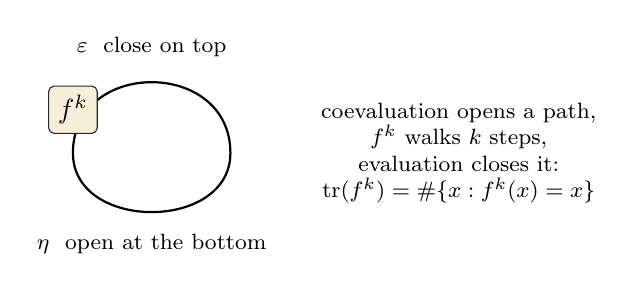
\begin{tikzpicture}[baseline]
\draw[thick] (0,0) .. controls (0,-1) and (2,-1) .. (2,0);
\draw[thick] (0,0) .. controls (0,1.2) and (2,1.2) .. (2,0);
\node[draw=ink,fill=faceF!15,rounded corners=2pt,minimum size=6mm] at (0,0.55) {$f^{k}$};
\node[font=\footnotesize] at (1,1.35) {$\varepsilon$ \ close on top};
\node[font=\footnotesize] at (1,-1.15) {$\eta$ \ open at the bottom};
\node[font=\footnotesize,align=center] at (4.9,0)
  {coevaluation opens a path,\\ $f^{k}$ walks $k$ steps,\\ evaluation closes it:\\
   $\tr(f^{k})=\#\{x:f^{k}(x)=x\}$};
\end{tikzpicture}
\end{center}

\noindent Only paths that can be closed survive; what returns is exactly the
round trips (fixed points of $f^{k}$; the Lefschetz slogan). The three recurring
bricks of the paper are this one move in three costumes.

\begin{center}
\renewcommand{\arraystretch}{1.35}
\begin{tabular}{@{}p{1.5cm} p{4.2cm} p{9.3cm}@{}}
\toprule
\textbf{Brick} & \textbf{Costume of the loop} & \textbf{In the paper / in Lean} \\
\midrule
\bF & \emph{the inserted map} --- one step $\sigma:x\mapsto x^{2}$
     (doubling $e\mapsto 2e$ on exponents) &
     the squaring behind every ``add the $2^{k}$-th power'' step;
     \lc{frob\_cycle}, \lc{frob\_mod}, \lc{frob\_bijective},
     \lc{pow\_field\_bijective}\ \ck \\
\bL & \emph{the closed loop itself} --- apply the loop to
     $m_{x}(y)=xy$ and it unwinds to $\Tr(x)=\sum_{i<n}x^{2^{i}}$ &
     states equation (1); telescope $L_m(x)^2{+}L_m(x)=x^{2^m}{+}x$;
     \lc{Tr}, \lc{truncTrace}, \lc{truncTrace\_sq\_add\_self},
     \lc{Tr\_eq\_algebraMap\_trace}\ \ck \\
\bC & \emph{the surviving loops} --- fixed points of $\sigma^{k}$; cycles
     of length dividing $k$ &
     cyclotomic cosets, reduced normal forms, $\gcdd(2^{k}{-}1,2^{n}{-}1)=1$;
     \lc{mersenne\_coprime}, \lc{inv\_mod\_exists}\ \ck \\
\bottomrule
\end{tabular}
\end{center}

\begin{verdict}\small\textbf{Why \bX\ is not a fourth brick.} For $K\subseteq L$
the field trace is $\Tr_{L/K}(x)=\tr(m_{x})$ --- the loop applied to
multiplication. Over $K=\FF_2$ this unwinds (Mathlib
\lc{FiniteField.algebraMap\_trace\_eq\_sum\_pow}) to $\sum_{i<n}x^{2^{i}}$, i.e.\
the project's own \bL. This identification is machine-checked
(\lc{Tr\_eq\_algebraMap\_trace}, \lc{Equation1/TraceLibrary.lean})\ \ck, so \bX\
is literally the hinge that makes \bL\ = ``sum around the \bF-orbit'' the genuine
field trace, not a fourth ingredient.
\end{verdict}

%======================================================================
\section{The extra hinge that reaches Sections 3--4: characters are eval/coeval too}

Sections 3--4 of the paper are about \emph{difference sets, autocorrelation and
2-rank}. At first sight these look like a different world from the trace loop.
They are not --- provided one notices that \emph{Fourier duality over $\FF_{2^n}$
is itself an evaluation/coevaluation}.

\begin{note}\small
The additive character $\psi(x)=(-1)^{\Tr(x)}$ is the canonical pairing
$L\otimes L\to \{\pm1\}$, $x\otimes y\mapsto(-1)^{\Tr(xy)}$ --- an
\emph{evaluation} identifying $L$ with its own Pontryagin dual, built directly on
the trace loop \bL. Consequently:
\begin{itemize}\setlength\itemsep{1pt}
\item A \emph{trace description} $\chi_{M}(x)=(-1)^{\Tr(p(x))}$ (Theorems 8, Cor
      12) is nothing but reading a set through this evaluation pairing.
\item The \emph{autocorrelation} of a sequence is
      $\sum_{x}(-1)^{\Tr(R(x)+R(ax))}$ --- the pairing of $R$ with its shift
      $R\circ(\times a)$, i.e.\ the \emph{trace of the translation operator}
      $T_a$. ``Ideal autocorrelation'' = this trace is flat (constant $-1$) for
      every $a\neq1$ = the round-trip/feedback of $T_a$ carries no extra memory.
\item ``$B^{*}$ is a \emph{difference set}'' is exactly that flatness, so it is a
      statement about the traces $\tr(T_a)$ of all nontrivial shifts.
\item The \emph{2-rank / linear span} $n\cdot w(p)+1$ counts the surviving
      cyclotomic cosets in $p$ --- brick \bC, the surviving loops --- so it, too,
      is a round-trip census.
\end{itemize}
\end{note}

\noindent With this hinge, the two halves of the paper share one vocabulary:
Section 2 is the loop applied to \emph{field maps} (permutation criteria),
Sections 3--4 the loop applied to \emph{shift operators on the group algebra}
(difference sets). Both are $\tr(f^{k})$ = ``what returns''.

\begin{caveat}\small The hinge \emph{expresses} the difference-set layer in the
trace language; it does not \emph{prove} it. Evaluating the shift-traces
$\sum_x(-1)^{\Tr(R(x)+R(ax))}$ to the difference-set value is exactly the hard
Gau\ss/Jacobi-sum work of Evans--Hollmann--Krattenthaler--Xiang and the
Dillon--Dobbertin difference-set proof. The pattern says \emph{what} to compute
(a trace of a shift); it does not compute it.
\end{caveat}

%======================================================================
\section{The paper, section by section, through the loop}

For each result: the categorical reading, the extra ingredient (if any), and the
Lean status.

\subsection*{\S2 \quad Permutation criteria and APN}

\textbf{Theorem 1 (Kasami $q_\alpha$ is a permutation $\iff k'+\alpha n\equiv1$).}
A polynomial is a permutation iff every fibre is a single round trip. The proof
reduces ``$q_\alpha(x)=$ const has $\le1$ solution'' by \emph{adding the
$2^{k}$-th power of equation (1) to itself} --- one application of \bF\ --- to the
linearized equation (2); the count of solutions is then a fixed-point/round-trip
count. Pure \bF+\bL, with \bC\ ($\gcdd(2^k{-}1,2^n{-}1)=1$) deciding solvability.
\hfill \lc{theorem\_1}, \lc{eqn2\_of\_eqn1}, \lc{theorem\_1\_case1},
\lc{theorem\_1\_case2}\ \ck

\textbf{Corollary 2 (Kasami power functions are APN).} $x^{d}$ is APN because
$p(t)=\tfrac1k q(t^{2^k}+t)$ and $t\mapsto t^{2^k}+t$ is two-to-one. The fibre of
the Artin--Schreier map has size $|\ker|=2^{\gcdd(k,n)}=2$ --- a subfield, the
fixed structure of \bF. So APN is ``the loop of $t\mapsto t^{2^k}+t$ closes on a
$2$-element orbit''. \emph{Reading: \bF.} \hfill \notlean\ (two-to-one map not in
this extract)

\textbf{Theorem 3 (MCM $P_\beta$).} The exact analogue for MCM polynomials; same
loop, same round-trip count. \hfill \notlean

\textbf{Theorem 4 (Kasami $\leftrightarrow$ MCM).} The correspondence
$\varphi_\alpha\psi_\beta=\id$ is a \emph{linearized change of costume}: the two
polynomial classes are the same underlying map dressed differently, and
$\psi_\beta,\varphi_\alpha$ are linearized (\bF+\bL) substitutions. This is
precisely the loop's conjugation-invariance $\tr(gfg^{-1})=\tr(f)$,
$\tr(gf)=\tr(fg)$ --- the categorical reason ``same map, two costumes'' is even
possible. \emph{Reading: \bX\ (basis-independence) + \bL.} \hfill \notlean

\subsection*{\S3 \quad Inverses, the trace description of $B$, and 2-rank}

\textbf{Theorem 5 ($q^{(\varepsilon)}$ is a permutation $\iff
\varepsilon\equiv k'+1$).} The trace-free twin of Theorem 1; the same
``add-the-$2^k$-power'' \bF\ telescope drives it. \hfill \lc{theorem\_5} and its
supporting layer (\lc{sTrace\_telescope\_gen}, \lc{root\_count},
\lc{qeps\_ne\_zero}, \dots)\ \ck

\textbf{Theorem 6 (inverse $q^{-1}(1/y)=R(y)$).} The elimination that produces
$R$ is \emph{iterated Frobenius}: at step $i$ one multiplies by powers of $y$ and
adds the $2^{ik}$-th power to kill $x^{2^{ik}}$ --- \bF\ applied again and again.
The surviving monomials of $R$ are indexed by cyclotomically inequivalent
exponents --- \bC. \emph{But} the bookkeeping of \emph{how many} survive obeys
$w(A_{i+2})=w(A_{i+1})+w(A_i)$: a genuine \textbf{Fibonacci recursion} that the
bare loop does not predict. \emph{Reading: \bF+\bC\ organise it; the recursion is
extra combinatorics.} \hfill \notlean

\textbf{Corollary 7 ($p^{-1}$ for MCM).} $p^{-1}=\varphi_0\circ R$ via Theorem 4;
same costume-change \bX\ composed with Theorem 6. \hfill \notlean

\textbf{Theorem 8 ($x\in B \iff \Tr(R(x))=0$).} This is the loop in its purest
applied form: membership of the image $B$ of $(x{+}1)^d+x^d+1$ is read off by a
single trace condition \bL\ on the inverse $R$. The trace layer that powers it
--- Frobenius-invariance of the trace $\Tr(x^{2^k})=\Tr(x)$, the Artin--Schreier
vanishing $\Tr(t^{2^k}+t)=0$, idempotence $\Tr(x)^2=\Tr(x)$, the bit property
$\Tr(x)\in\{0,1\}$, and the Case-1 criterion for the trace-version permutation
$g$ --- \emph{is} formalised. \emph{Reading: \bL\ (+\bF).} \hfill
\lc{trace\_frob\_shift}, \lc{trace\_artin\_schreier\_zero}, \lc{trace\_sq},
\lc{trace\_bit}, \lc{gmap\_bijective\_iff}\ \ck\ ; the full statement with $R$
itself \notlean

\textbf{Lemma 9 ($R$ reduced $\iff k'<n/2$; $w(R)=2F_{k'}-1$).} A statement about
\emph{which round trips survive} (cyclotomic non-equivalence, \bC) and how many
(\bF ibonacci again). \emph{Reading: \bC\ + the Fibonacci extra.} \hfill \notlean

\textbf{Corollaries 10, 11 (2-rank $=n(2F_{k'}-1)+1$; Segre 2-rank).} The 2-rank
is $n\cdot w(R)+1$ = (coset count) --- a census of surviving loops \bC, read
through the character pairing of \S2. The actual value uses Lemma 9 (Fibonacci)
and, for the confirmation, Gau\ss/Jacobi sums. \hfill \notlean

\textbf{Corollary 12 (No--Chung--Yun trace expansion).} A concrete trace
description $\chi_N(x)=(-1)^{\Tr(S_i(x))}$ with $S_i$ built from explicit
cyclotomic-coset exponents. \emph{Reading: \bL\ (character) + \bC\ (cosets).}
\hfill \notlean

\subsection*{\S4 \quad The difference-set conjecture (now a theorem)}

\textbf{Conjecture / Theorem (Dillon--Dobbertin): $B^{*}$ is a cyclic difference
set.} Equivalent to $\sum_{x}(-1)^{\Tr(R(x)+R(ax))}=0$ for all $a\neq1$: the
\emph{trace of every nontrivial shift $T_a$ is flat}. This is the eval/coeval
loop applied to the translation operators on the group algebra (the hinge of
\S2 above). \emph{Reading: \bX/\bL\ over the group algebra --- but the proof is
Gau\ss/Jacobi-sum evaluation, genuinely beyond the bare pattern.} \hfill \notlean

%======================================================================
\section{Master table}

\begin{center}
\renewcommand{\arraystretch}{1.25}
\begin{tabular}{@{}p{3.4cm} p{3.1cm} p{5.2cm} p{2.6cm}@{}}
\toprule
\textbf{Result} & \textbf{Loop facet} & \textbf{Extra ingredient beyond the bare
pattern} & \textbf{Lean} \\
\midrule
Thm 1 (Kasami PP) & \bF\ insert, \bL\ close, \bC\ solvable & --- (the pattern
essentially gives it) & \ck\ \lc{theorem\_1} \\
Cor 2 (APN) & \bF\ (2-to-1 kernel) & the $t\mapsto t^{2^k}{+}t$ substitution &
\notlean \\
Thm 3 (MCM PP) & same loop & --- & \notlean \\
Thm 4 (Kasami$\leftrightarrow$MCM) & \bX\ conjugation-inv. & the explicit
linearized change of variable & \notlean \\
Thm 5 ($q^{(\varepsilon)}$ PP) & \bF+\bL & --- & \ck\ \lc{theorem\_5} \\
Thm 6 (inverse $R$) & \bF\ iterated, \bC & \textbf{Fibonacci recursion}
$A_{i+2}{=}A_{i+1}{+}A_i$ & \notlean \\
Cor 7 ($p^{-1}$) & \bX\ + Thm 6 & --- & \notlean \\
Thm 8 ($x\in B\iff\Tr R(x){=}0$) & \bL\ (+\bF) & the inverse $R$ itself & \ck\
trace layer \\
Lemma 9 (reduced, $w{=}2F_{k'}{-}1$) & \bC & Fibonacci & \notlean \\
Cor 10/11 (2-rank) & \bC\ census, \bL\ pairing & Fibonacci + Gau\ss/Jacobi sums &
\notlean \\
Cor 12 (No--Chung--Yun) & \bL\ char., \bC\ cosets & explicit exponent
bookkeeping & \notlean \\
\S4 (difference set) & \bX/\bL\ over group algebra & Gau\ss/Jacobi-sum evaluation
& \notlean \\
\bottomrule
\end{tabular}
\end{center}

%======================================================================
\section{Verdict}

\begin{verdict}
\textbf{Does one categorical pattern underlie the whole paper?} As a
\emph{unifying language}: yes, and more completely than one might expect. Every
device the paper leans on is the single eval/coeval move in a costume ---
\bF\ inserts, \bL\ closes, \bC\ are the survivors --- and even Sections 3--4,
which look combinatorial, run on the character $\psi=(-1)^{\Tr}$, itself the
evaluation pairing built on \bL; a difference set is then the flatness of the
trace of every nontrivial shift. The loop tells you, uniformly, \emph{what to
look at}: round trips, fixed points, surviving cosets, flat shift-traces.
\end{verdict}

\begin{caveat}
\textbf{But it is a lens, not a machine.} Three places carry mathematics the bare
pattern does not hand you: (i) the \emph{Fibonacci recursion} governing the
inverse $R$ and its weight $w(R)=2F_{k'}-1$ (Theorem 6, Lemma 9); (ii) the
\emph{Gau\ss/Jacobi-sum} evaluation behind the 2-rank and the difference-set
proof (Corollaries 10/11, Section 4); (iii) the specific \emph{linearized change
of variable} realising Kasami$\leftrightarrow$MCM (Theorem 4). The pattern
organises and motivates all of these, but each needs its own argument. And in
\emph{this} formalisation the loop appears in its concrete Frobenius/field-trace
form (\lc{Tr\_eq\_algebraMap\_trace}), not as literal string diagrams: what is
machine-checked \ck\ is the Theorem-1/Theorem-5 permutation tower and the
Theorem-8 trace layer; the difference-set half is outside the extract.
\end{caveat}

\vfill
\begin{center}\footnotesize
Companion to \texttt{PaperStory.tex}, \texttt{Equation1\_LEGO.tex},
\texttt{TraceMap\_Categorically.tex}, \texttt{TracePowers\_Relations.tex},
\texttt{TraceAsMemory.tex}.\\
Source: \emph{Dobbertin, Kasami Power Functions, Permutation Polynomials and
Cyclic Difference Sets} (1999). Rebuild: \texttt{tectonic
Dobbertin\_OneCategoricalPattern.tex}.
\end{center}

\end{document}
